\chapter{The predictor/corrector integration scheme}

\begin{figure}[]
  \centering
  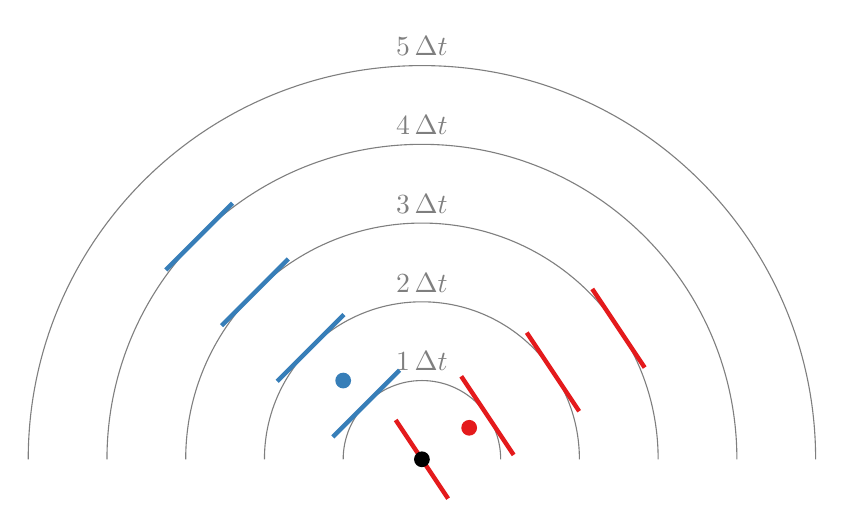
\begin{tikzpicture}[scale=1.0]

  \definecolor{Set1-3-1}{RGB}{228,26,28}
  \definecolor{Set1-3-2}{RGB}{55,126,184}

  \foreach \i in {1,2,3,4,5} {
    \draw[opacity=0.5] (\i, 0) arc (0:180:\i);
    \node[above, opacity=0.5] at (0, \i) {$\i \, \Delta t$};
  }

  \fill[color=Set1-3-1] (0.6, 0.4) circle (0.1);
  \begin{scope}[rotate=33.6901]
    \foreach \i in {0,1,2,3} {
      \draw[ultra thick, Set1-3-1] (\i,-0.6) -- (\i, 0.6);
    }
  \end{scope}


  \fill[Set1-3-2] (-1, 1) circle (0.1);
  \begin{scope}[rotate=135]
    \foreach \i in {1,2,3,4} {
      \draw[ultra thick, Set1-3-2] (\i,-0.6) -- (\i, 0.6);
    }
  \end{scope}

  \fill[black] (0, 0) circle (0.1);

  \end{tikzpicture}
  \caption{\label{fig:retardation problem} Illustration of the ``retardation problem'' in solving coupled delay differential equations.
    The filled points show particle locations and the colored tangent lines indicate historical quantities of $\vb{P}$  used in the interpolation scheme developed in \cref{ch:quantum dots}. 
    Because $\abs{\vb{r}_{\bullet \textcolor[RGB]{228,26,28}{\bullet}}} < c \, \Delta t$, determining $\qty{\vb{E}(\bullet, t),\vb{P}(\textcolor[RGB]{228,26,28}{\bullet}, t)}$ requires knowledge of $\qty{\vb{P}(\textcolor[RGB]{228,26,28}{\bullet}, t), \vb{E}(\bullet, t)}$.
  }
\end{figure}

\begin{figure}
  \centering
  \begin{subfigure}{0.4\textwidth}
    \centering
    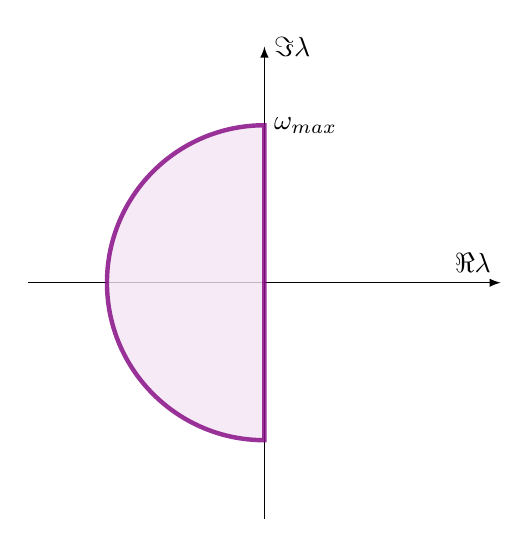
\begin{tikzpicture}[>=latex]
      \draw[->] (0,-3) -- (0, 3) node[right] {$\Im \lambda$};
      \draw[->] (-3,0) -- (3, 0) node[anchor=south east] {$\Re \lambda$};

      \draw[ultra thick, violet, fill=violet!10, opacity=0.8] (0,2) arc(-90:90:-2) -- (0,2) -- cycle;
      \node[right] at (0, 2) {$\omega_\text{max}$};
    \end{tikzpicture}
    \caption{\label{fig:filled semidisk}}
  \end{subfigure}
  \hspace{1cm}
  \begin{subfigure}{0.4\textwidth}
    \centering
    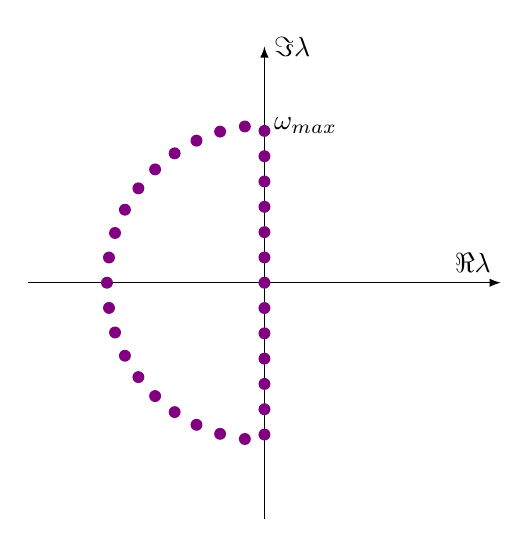
\begin{tikzpicture}[>=latex]
      \draw[->] (0,-3) -- (0, 3) node[right] {$\Im \lambda$};
      \draw[->] (-3,0) -- (3, 0) node[anchor=south east] {$\Re \lambda$};

      \foreach \point in {{0.,0.},{0.,0.32135},{0.,0.642699},{0.,0.964049},{0.,1.2854},{0.,1.60675},{0.,1.9281},{-0.248801,1.98446},{-0.563079,1.9191},{-0.862852,1.8043},{-1.1404,1.64301},{-1.38856,1.43941},{-1.60096,1.19872},{-1.77212,0.927148},{-1.89762,0.631695},{-1.97424,0.319969},{-2.,1.22465*10^-16},{-1.97424,-0.319969},{-1.89762,-0.631695},{-1.77212,-0.927148},{-1.60096,-1.19872},{-1.38856,-1.43941},{-1.1404,-1.64301},{-0.862852,-1.8043},{-0.563079,-1.9191},{-0.248801,-1.98446},{0.,-1.9281},{0.,-1.60675},{0.,-1.2854},{0.,-0.964049},{0.,-0.642699},{0.,-0.32135}}
      {
        \fill[violet] (\point) circle (0.5ex);
      }
      \node[right] at (0, 2) {$\omega_\text{max}$};
    \end{tikzpicture}
    \caption{\label{fig:discrete semidisk}}
  \end{subfigure}
  \caption{\label{fig:semidisk} Selection of the $\lambda_n$ parameters used in determining the predictor/corrector coefficients.
    The maximum modulus principle ensures that weights determined from $\lambda_n$ on the boundary of the semidisk incur the maximum approximation error, thus the numerical solution accurately recovers all modes with exponents within the semidisk.
  }
\end{figure}

\section{Motivation}

In principle, any standard numerical ODE solver will work just fine for integrating \cref{eq:liouville,eq:rotating liouville} for a single quantum system.
The retarded coupling between systems introduced by \cref{eq:integral operator,eq:radiated envelope} produces a set of coupled delay differential equations that imposes significant constraints on the structure of the ODE solver.
In particular,
\begin{inparaenum}[(i)]
  \item the geometry of any substantial system will have nonintegral retardation factors between pairs of particles (i.e.\ $\Delta r/(c \, \Delta t) \not \in \mathbb{Z}$) and
  \item we wish to accurately account for interactions between particles within $c \, \Delta t$ of each other given that we may use large timesteps with a rotating-wave approximation.
\end{inparaenum}
